\documentclass[border=6pt]{standalone}
\usepackage{tikz}
\usetikzlibrary{arrows.meta,positioning,calc,shapes.geometric}
\begin{document}
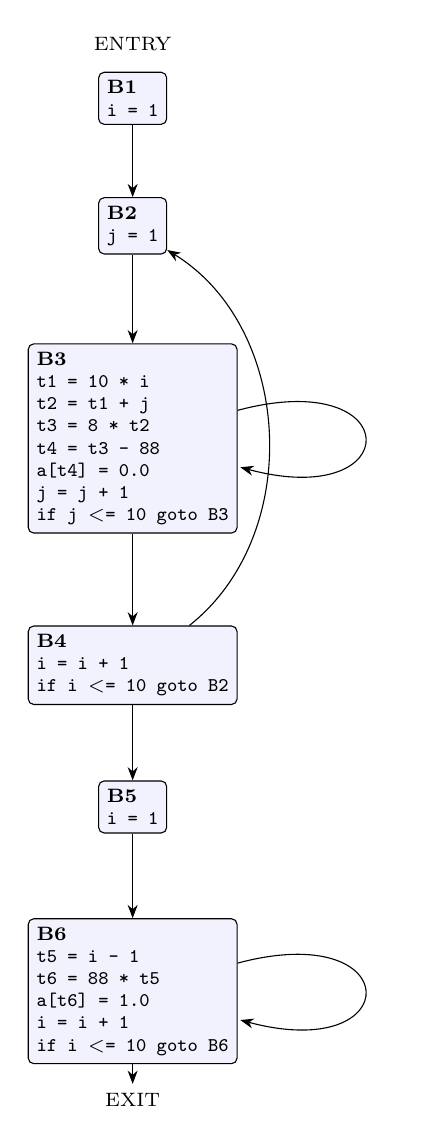
\begin{tikzpicture}[>=Stealth,font=\scriptsize,x=1.000cm,y=1.000cm,
 box/.style={draw,rounded corners=2pt,align=left,inner sep=3pt,fill=blue!5},
 circ/.style={draw,circle,align=center,inner sep=1pt,minimum size=0.75cm,fill=blue!5},
 lab/.style={font=\scriptsize,inner sep=1pt,fill=white,fill opacity=0.85,text opacity=1}]
\node[box] (b1) at (0.000,0.000) {\textbf{B1}\\\texttt{i = 1}};
\node[box] (b2) at (0.000,-1.620) {\textbf{B2}\\\texttt{j = 1}};
\node[box] (b3) at (0.000,-4.320) {\textbf{B3}\\\texttt{t1 = 10 * i}\\\texttt{t2 = t1 + j}\\\texttt{t3 = 8 * t2}\\\texttt{t4 = t3 - 88}\\\texttt{a[t4] = 0.0}\\\texttt{j = j + 1}\\\texttt{if j \textless{}= 10 goto B3}};
\node[box] (b4) at (0.000,-7.200) {\textbf{B4}\\\texttt{i = i + 1}\\\texttt{if i \textless{}= 10 goto B2}};
\node[box] (b5) at (0.000,-9.000) {\textbf{B5}\\\texttt{i = 1}};
\node[box] (b6) at (0.000,-11.340) {\textbf{B6}\\\texttt{t5 = i - 1}\\\texttt{t6 = 88 * t5}\\\texttt{a[t6] = 1.0}\\\texttt{i = i + 1}\\\texttt{if i \textless{}= 10 goto B6}};
\draw[->] (b1) --  (b2);
\draw[->] (b2) --  (b3);
\path[->] (b3) edge[loop right]  (b3);
\draw[->] (b3) --  (b4);
\draw[->] (b4) to[bend right=55]  (b2);
\draw[->] (b4) --  (b5);
\draw[->] (b5) --  (b6);
\path[->] (b6) edge[loop right]  (b6);
\node[font=\scriptsize,above=0.15cm of b1] {ENTRY};
\node[font=\scriptsize,below=0.25cm of b6] {EXIT};
\draw[->] (b6.south) -- ++(0,-0.25);
\end{tikzpicture}
\end{document}
